
\begin{center}
\thispagestyle{empty}

\vspace{.7cm}

% 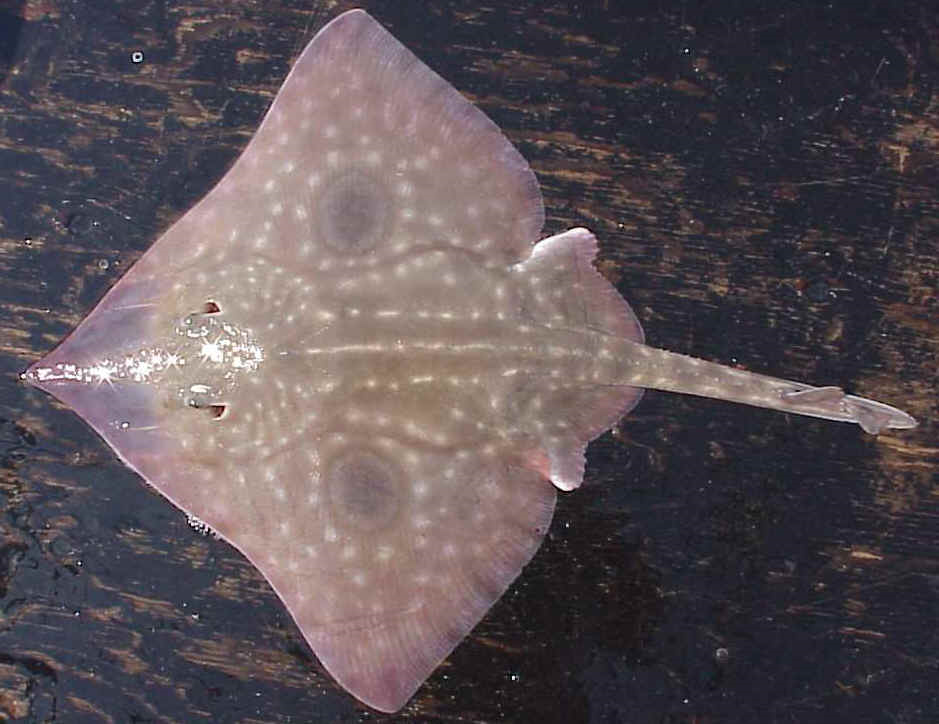
\includegraphics{cover_photo}~\\[1cm]
\pdftooltip{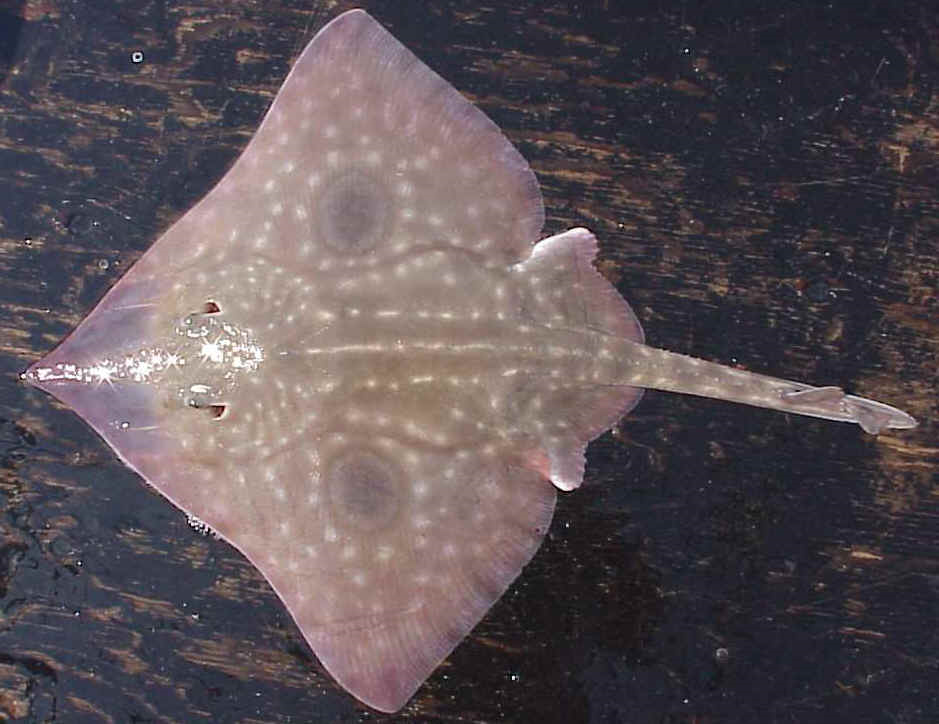
\includegraphics{cover_photo}}{This is a fish.}

\vspace{.5cm}

Ian G. Taylor\textsuperscript{1}\\
Vladlena Gertseva\textsuperscript{1}\\
Joseph Bizzarro\textsuperscript{2}\\
Andi Stephens\textsuperscript{3}\\

\vspace{.7cm}

\small

\textsuperscript{1}Northwest Fisheries Science Center, U.S. Department of Commerce, National Oceanic and Atmospheric Administration, National Marine Fisheries Service, 2725 Montlake Boulevard East, Seattle, Washington 98112\\

\vspace{.3cm}

\textsuperscript{2}Southwest Fisheries Science Center, U.S. Department of Commerce, National Oceanic and Atmospheric Administration, National Marine Fisheries Service, 110 Shaffer Road, Santa Cruz, California 95060\\

\vspace{.3cm}

\textsuperscript{3}Northwest Fisheries Science Center, U.S. Department of Commerce, National Oceanic and Atmospheric Administration, National Marine Fisheries Service, 2032 S.E. OSU Drive Newport, Oregon 97365


\vspace{.5cm}

\vfill
DRAFT SAFE\\
Disclaimer: This information is distributed solely for the purpose of pre-dissemination
peer review under applicable information quality guidelines. It has not been formally
disseminated by NOAA Fisheries. It does not represent and should not be construed to
represent any agency determination or policy. 

\vspace{.3cm}
%Bottom of the page
%{\large \today}


\newpage{\thispagestyle{empty}}

\vspace*{\fill}
\begin{flushleft}
This report may be cited as:

Taylor, I.G., Gertseva, V., Bizzarro, J., and Stephens, A. Status of Big Skate (\emph{Beringraja binoculata}) Off the U.S. West Coast, 2019. Pacific Fishery Management Council, Portland, OR. Available from http://www.pcouncil.org/groundfish/stock-assessments/
\end{flushleft}

\maketitle

\pagenumbering{roman}
\setcounter{page}{1}
\end{center}


